\chapter[Testy i eksperymenty]{Testy i eksperymenty}
\label{chapter:testy}
Wszystkie testy w tym rozdziale zostały przeprowadzone na czterokanałowym oscyloskopie marki Hantek \cite{hantek}. 
Dołożono wszelkich starań, by wyniki eksperymentów były powtarzalne i przedstawione w możliwe łatwy do zinterpretowania sposób.
Ze względu na charakterystykę pomieszczenia, w którym dokonywano pomiarów, wyniki mogą być obarczone dużym błędem. 
Ma na to wpływ ilość obiektów oraz powierzchni odbijających dźwięk.


\section{Test przetwornika piezoelektrycznego}
Pierwszym testem był test przetwornika, który jest nadajnikiem sygnału. Zasilono go bezpośrednio z generatora wbudowanego w oscyloskop, 
parametry zadane to sygnał sinusoidalny o napięciu \unit[5]{V} \textit{peak-to-peak}, czyli wartości szczytowej.
Elementem odbiorczym był inny przetwornik piezoelektryczny służący tylko do testów. Jego częstotliwość rezonansowa również wynosiła \unit[40]{kHz}.
Przetworniki zostały skierowane w tym samym kierunku, tak by do odbiornika dotarł dźwięk odbity od powierzchni przedmiotu. 
Odległość od tego przedmiotu wyniosła około \unit[25]{cm}, a stanowisko zostało przedstawione na rysunku \ref{fig:oscylo_piezo_photo}.
Po podłączeniu sondy oscyloskopu do odbiornika ukazał się wyraźny sygnał w kształcie sinusoidy ustawionej na nadajniku.
Dźwięki otoczenia miały bardzo znikomy wpływ na zakłócenia, stanowiąc niewielki procent amplitudy. 
Zmiana częstotliwości o chociażby \unit[1]{kHz} wiązała się kilkudziesięciokrotnym spadkiem mocy sygnału, co potwierdzało dane z noty katalogowej elementu piezoelektrycznego.
Na rysunku \ref{fig:oscylo_piezo} kolorem czerwonym ukazany jest sygnał podawany na nadajnik, zaś kolorem niebieskim zaznaczono sygnał bezpośrednio z odbiornika.
Sprawdzono również wpływ odległości czujników na moc i przesuniecie fazy sygnału.
Zmieniając odległość nadajnika od odbiornika dało się w czasie rzeczywistym zauważyć przesuwanie się fazy sygnału oraz zmianę jego amplitudy. 

\begin{figure}[!ht]
    \centering
    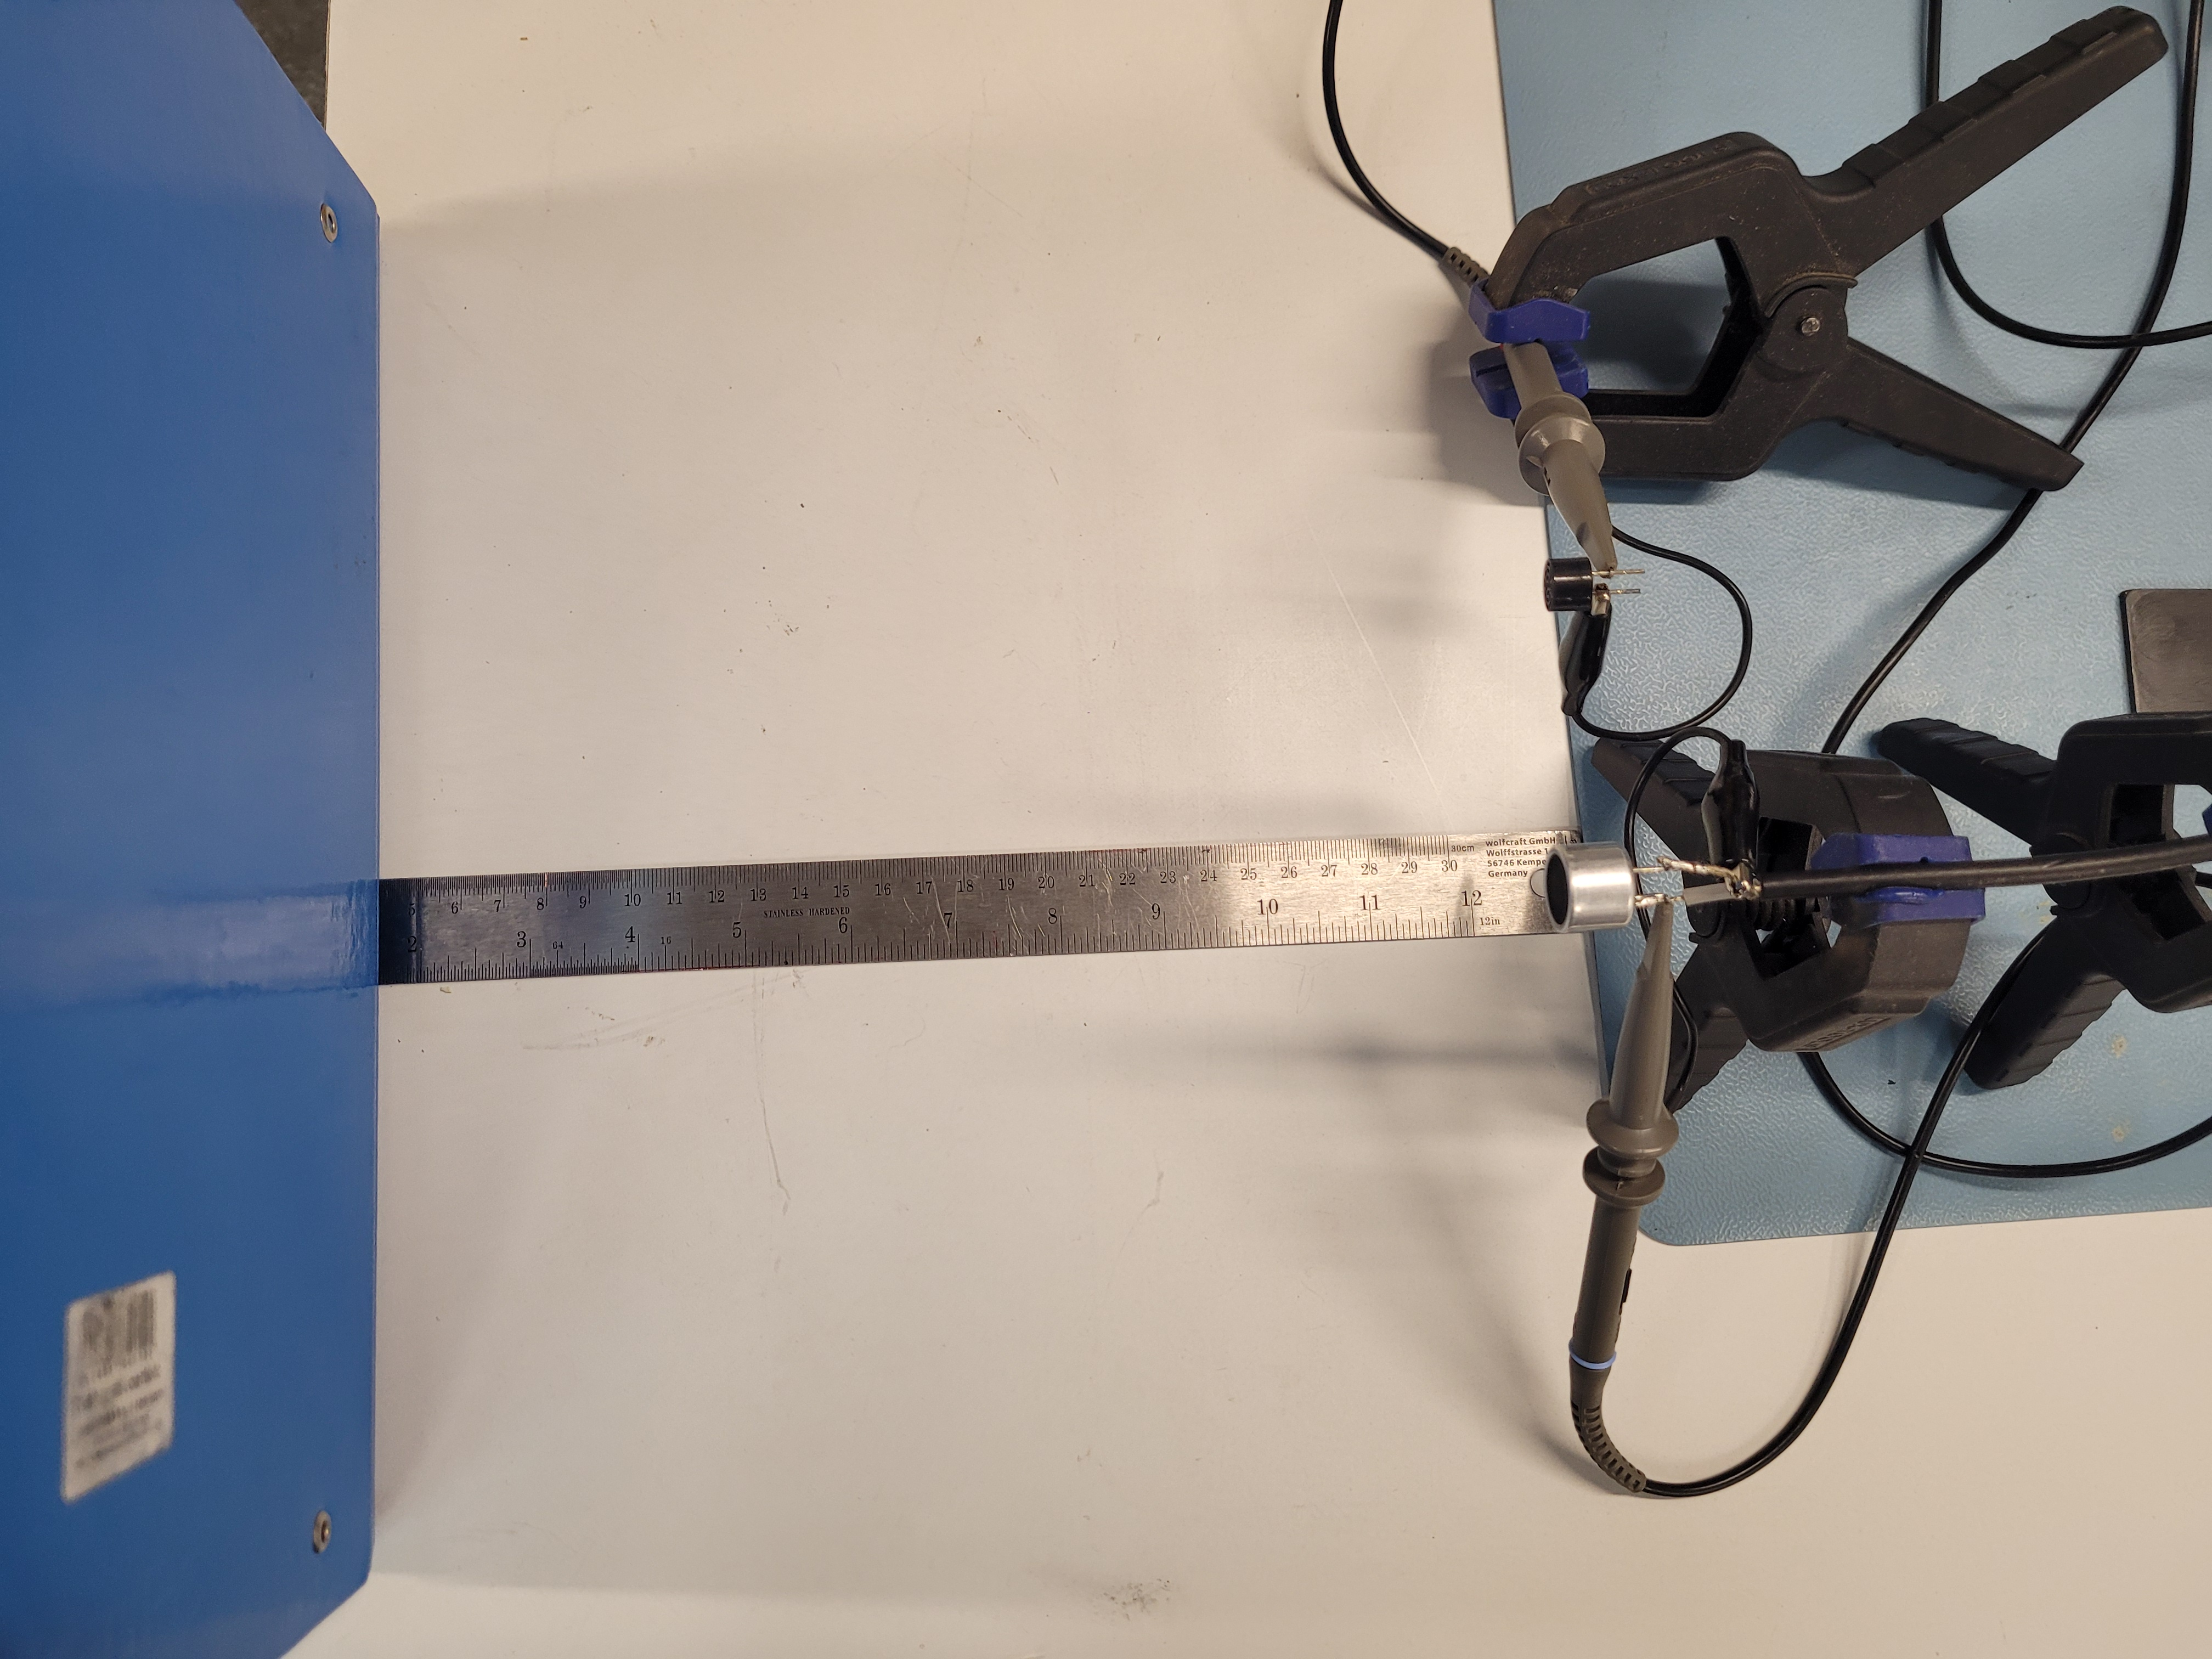
\includegraphics[ width = 0.4\textwidth]{20221214_122856.jpg}
    \caption{Stanowisko badawcze}
    \label{fig:oscylo_piezo_photo}
\end{figure}

\begin{figure}[!ht]
    \centering
    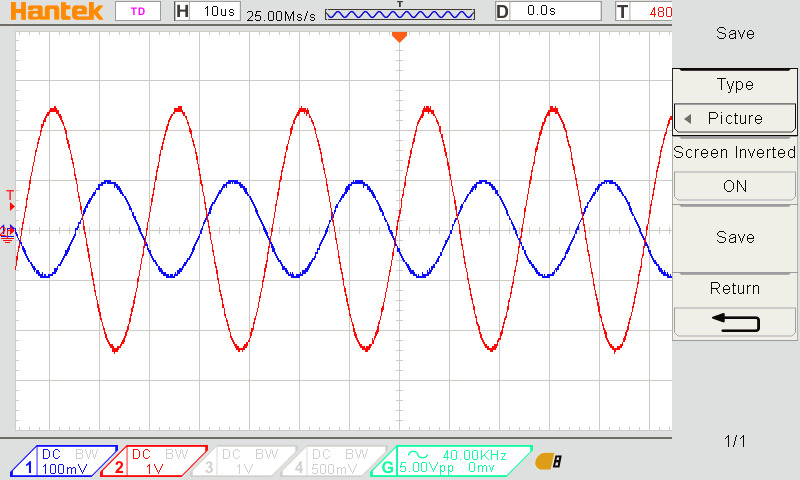
\includegraphics[width = 0.4\textwidth]{piezo_piezo.jpg}
    \caption{Przebieg sygnału odebrany innym przetwornikiem piezoelektrycznym}
    \label{fig:oscylo_piezo}
\end{figure}

\section{Pierwsze uruchomienie}
PCB z przylutowanymi elementami zostało podłączone do zasilacza laboratoryjnego dostarczającego \unit[5]{V} i ograniczeniem prądowym ustawionym na \unit[100]{mA}. 
Pierwsze uruchomienie sterownika sonaru ujawniło drobny błąd projektowy, wszystkie diody elektroluminoescencyjne zostały przylutowane w złej polaryzacji.
Zmiana ustawień diod i następne uruchomienie, nie pokazywało oznak większych błędów. Pobór prądu wyniósł około \unit[30]{mA}, a temperatura elementów na 
płytce nie odbiegała od temperatury pokojowej.

\section{Uruchomienie i test wzmacniacza sygnału przetwornika piezoelektrycznego}
Wzmacniacz nadajnika zachował się zgodnie z założeniami projektowymi. Podając impuls o wartości napięcia \unit[5]{V} otrzymano na wyjściu transformatora \unit[80]{V} peak-to-peak. 
Na rysunku \ref{fig:amplifier} kolorem czerwonym oznaczono sygnał za tranzystorem kluczującym, a kolorem cyjanowym sygnał na wyjściu transformatora.

\begin{figure}[!ht]
    \centering
    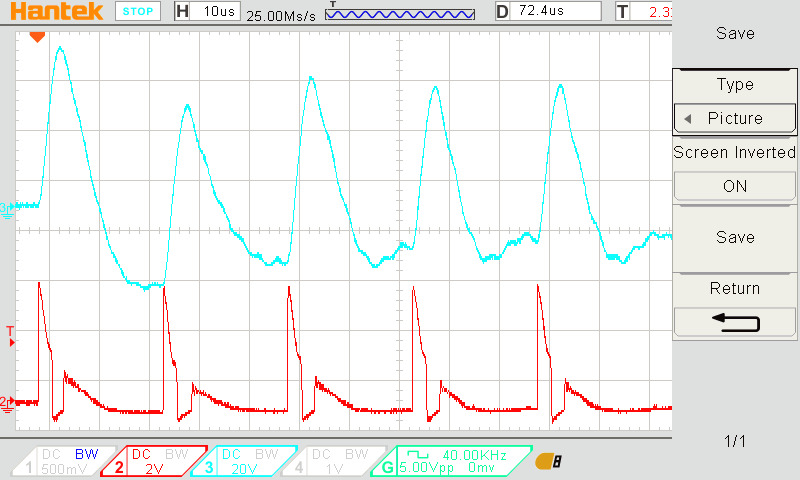
\includegraphics[width = 0.5\textwidth]{piezo_oscylo.jpg}
    \caption{Wyjście transformatora z podłączonym przetwornikiem piezoelektrycznym}
    \label{fig:amplifier}
\end{figure}

\section{Test mikrofonów i filtrów}
Następnym testem było sprawdzenie, jak na poszczególnych etapach analogowego przetwarzania zachowuje się sygnał odbierany z mikrofonów. 
Przetestowanie poziomu napięć z mikrofonu wykazało, że jest on większy niż zakładano. 
Najlepszą amplitudę sygnału uzyskano za drugim filtrem częstotliwości. Z tym poziomem wzmocnienia sygnał z nadajnika był bardzo wyraźny i 
rzadko przesterowany. Jednocześnie szumy i zakłócenia były na tyle niskie, by nie mieć negatywnego wpływu na jakość sygnału. 
Z tego powodu trzeci stopień wzmocnienia został całkowicie pominięty mostkiem na płytce obwodu drukowanego. 
Na rysunku \ref{fig:mic_amp_comp} widać przebiegi sygnałów:
\begin{itemize}
    \item na niebiesko -- surowy sygnał z mikrofonu,
    \item na czerwono -- przefiltrowany i wzmocniony sygnał,
    \item na cyjanowo -- sprogowany sygnał przez komparator, gotowy do odczytu przez mikrokontroler.
\end{itemize} 
Jak wynika z pomiarów, rzeczywisty poziom wzmocnienia filtrów częstotliwości wyniósł \unit[40]{V/V}. Wzmacniacz operacyjny wprowadził do sygnału 
zauważalne przesunięcie fazowe, jednakże w tym zastosowaniu nie ma to negatywnego wpływu na działanie układu. Wartość progowania komparatora
została ustawiona na \unit[1,65]{V}, czyli taka sama jak punkt pracy filtrów. Na rysunku \ref{fig:mic_amp_comp} widać punkt przecięcia wykresów czerwonego i cyjanowego. 
Wyznacza on wartość napięcia progowania, która zgadza się z zadaną wartością, co świadczy o prawidłowym funkcjonowaniu komparatora.  


\begin{figure}[!ht]
    \centering
    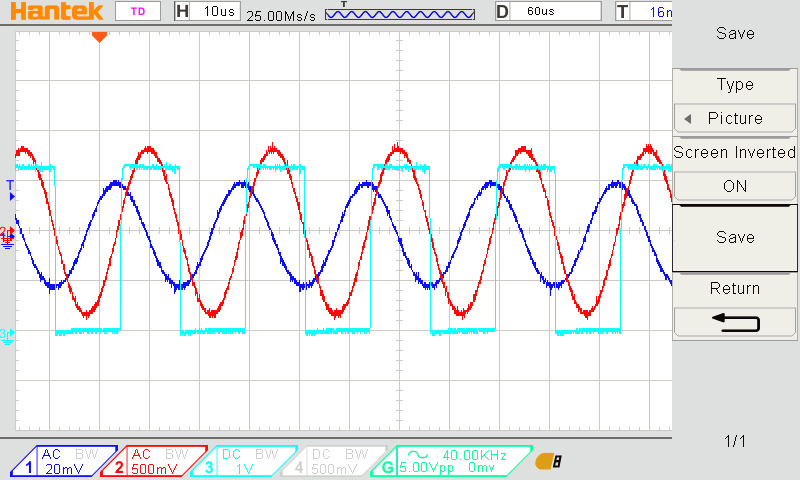
\includegraphics[width = 0.5\textwidth]{mic_amp_comp.jpg}
    \caption{Przebiegi sygnałów z pojedynczego kanału w punkcie pomiaru kolejno za mikrofonem, wzmacniaczem i komparatorem}
    \label{fig:mic_amp_comp}
\end{figure}

\section{Test wykrywania obiektu}
Najważniejszym testem mającym potwierdzać główne założenie projektu jest wykrycie pozycji obiektu, co okazało się być skomplikowanym zadaniem. 
Ze względu na echo sygnału, trudno było znaleźć dokładny okres fali, który odbity został od wyznaczonego przedmiotu.
Na rysunkach \ref{fig:bezobiektu} i \ref{fig:zobiektem} przedstawiono wzmocnione sygnały z trzech mikrofonów jednocześnie. 
Zarówno w przypadku obecności badanego obiektu, jak i bez w celu porównania. 
W okolicy dziewiątego okresu widać istotne załamanie, które może świadczyć właśnie o pojawieniu się przedmiotu. 
Obiekt postawiono w odległości około \unit[4]{cm} od nadajnika (patrz rys. \ref{fig:stanowisko}), ze względu na krótki bufor pomiaru. 
Mierzenie dłuższego okna czasowego miałoby istotny wpływ na jakość danych wyświetlanych na ekranie oscyloskopu.

\begin{figure}[!ht]
    \centering
    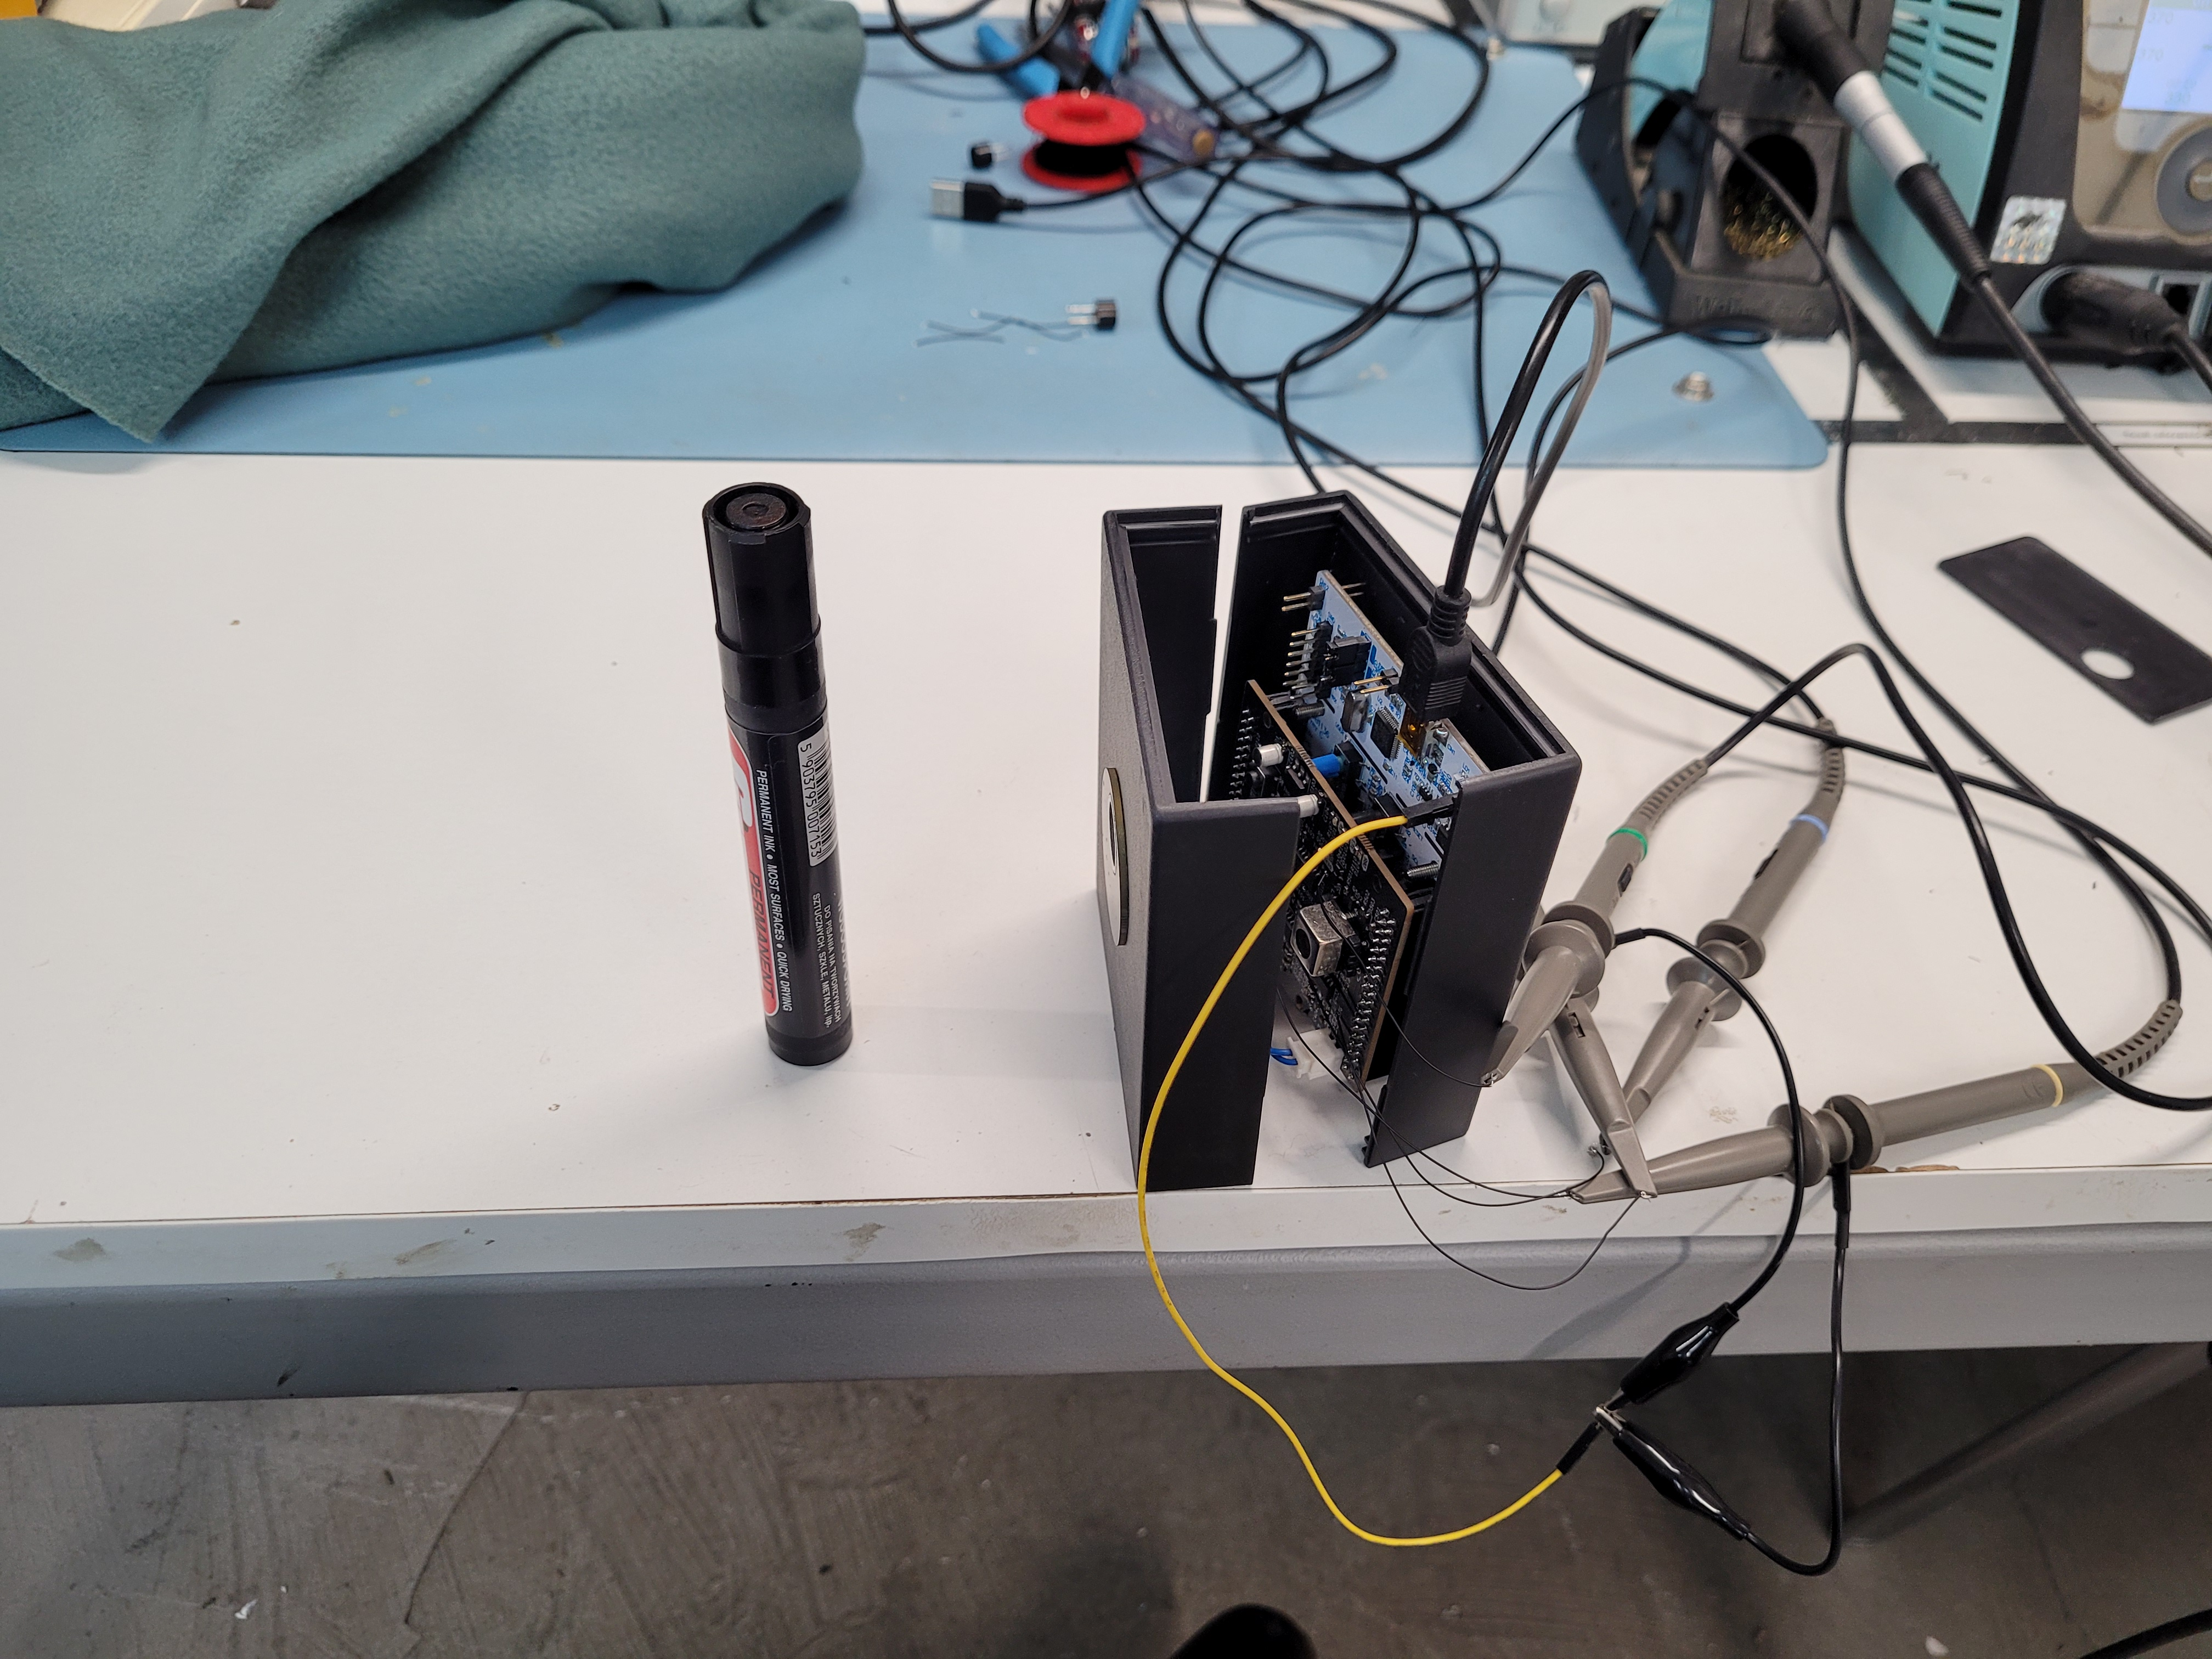
\includegraphics[trim={20cm 20cm 20cm 20cm},clip , width = 0.5\textwidth]{20221221_163955.jpg}
    \caption{Stanowisko badawcze wykrywania obiektu}
    \label{fig:stanowisko}
\end{figure}

W pierwszych okresach przebiegu sygnału widać przesunięcie fazowe. 
Te okresy prawdopodobnie wynikają z bezpośredniego oddziaływania przetwornika na mikrofony, które leżą od niego w różnej odległości.  


\begin{figure}[!ht]
    \centering
    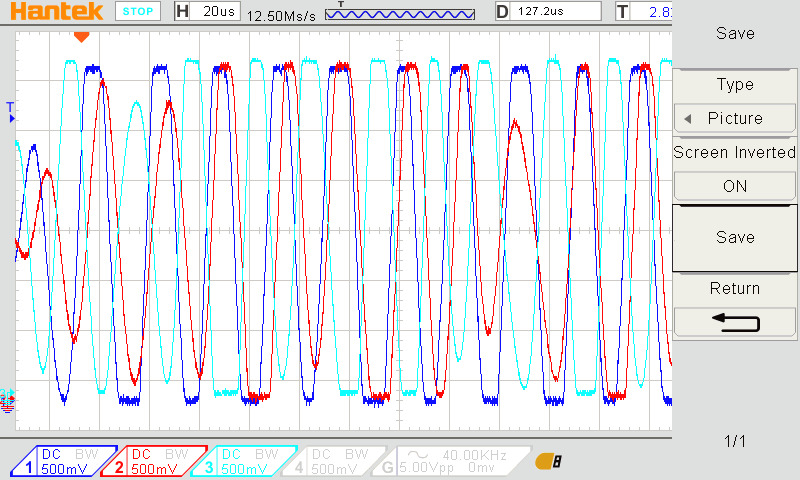
\includegraphics[width = 0.7\textwidth]{dso_12_22_01_00_32.jpg}
    \caption{Odebrany sygnał bez badanego obiektu}
    \label{fig:bezobiektu}
\end{figure}

\begin{figure}[!ht]
    \centering
    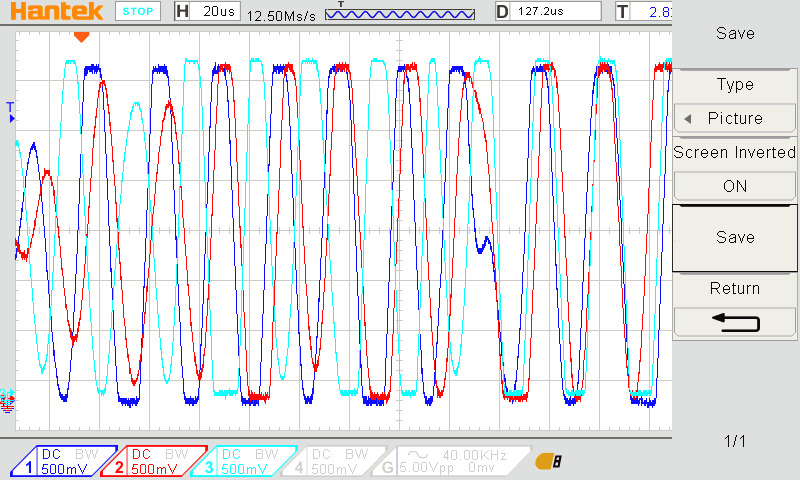
\includegraphics[width = 0.7\textwidth]{dso_12_22_01_00_49.jpg}
    \caption{Odebrany sygnał z badanym obiektem}
    \label{fig:zobiektem}
\end{figure}

